\chapter{Sistemi Multiagente}

\qs{}{Perché sistemi distribuiti di agenti?}

\begin{itemize}
  \item Le soluzioni centralizzate sono spesso impraticabili perché i sistemi e i dati coinvolti appartengono a organizzazioni indipendenti. 
  \item Le informazioni coinvolte sono distribuite e risiedono in sistemi informativi di grosse dimensioni e complessi sotto diversi punti di vista:
    \begin{itemize}
      \item Distribuiti geograficamente.
      \item Composti da molte parti indipendenti. 
      \item Contenuti di grandi dimensioni. 
      \item Coprono una porzione maggiore del dominio considerato.
    \end{itemize}
\end{itemize}

\paragraph{Ci sono quattro tecniche principali per affrontare la \fancyglitter{dimensione} e la \fancyglitter{complessità} di un sistema informativo:}

\begin{itemize}
  \item Modularità. 
  \item Distribuzione. 
  \item Astrazione. 
  \item Intelligenza.
\end{itemize}

\nt{L'uso di moduli distribuiti Intelligenti combinati a queste tecniche produce un approccio di \fancyglitter{intelligenza artificiale distribuita} (DAI). Gli agenti fanno parte di questo approccio.}

\dfn{Sistemi Autonomi di Agenti}{
  Per lo sviluppo di soluzioni globali e distribuite gli agenti necessitano di essere eseguiti in maniera autonoma e sviluppati indipendentemente. Gli agenti coordinano, cooperano e, eventualmente, competono per la soluzione di problemi, condividendo capacità e lavorando in parallelo. Questo porta ai sistemi Multiagente.
}

\nt{Sistemi autonomi rappresentano soluzioni modulari e riutilizzabili.}

\qs{}{Perché comunicare?}

\begin{itemize}
  \item Gli agenti operano in ambienti che contengono altri agenti.
  \item Un sistema multiagente è un sistema che contiene agenti che interagiscono tra di loro attraverso la \fancyglitter{comunicazione}. 
  \item Hanno le seguenti caratteristiche:
    \begin{itemize}
      \item Forniscono un'infrastruttura specifica per la comunicazione e l'utilizzo di protocolli di interazione. 
      \item Sono progettati per essere \fancyglitter{aperti} e \fancyglitter{distribuiti}. 
      \item Gli agenti ospitati sono \fancyglitter{autonomi}, \fancyglitter{self-interested} o \fancyglitter{cooperativi}.
    \end{itemize}
  \item Le infrastrutture includono:
    \begin{itemize}
      \item \fancyglitter{Protocolli di comunicazione:} per permettere agli agenti di comprendere i messaggi scambiati. 
      \item \fancyglitter{Protocolli di interazione:} per permettere agli agenti di svolgere conversazioni, ossia scambi strutturati di messaggi. 
    \end{itemize}
  \item Gli agenti coordinano le loro azioni e i loro comportamenti. Quest'abilità è parte della percezione (ricevere messaggi) e parte delle azioni (inviare messaggi). 
  \item La \fancyglitter{coordinazione} è una proprietà di un sistema di agenti che eseguono attività in un ambiente condiviso. 
  \item La \fancyglitter{cooperazione} è coordinazione tra agenti non antagonisti. 
  \item La \fancyglitter{negoziazione} è coordinazione tra agenti antagonisti, competitivi o self-interested.
\end{itemize}

\paragraph{Un protocollo di comunicazione potrebbe includere i seguenti tipi di messaggio:}

\begin{itemize}
  \item Proposta di esecuzione di un'azione. 
  \item Accettare una proposta. 
  \item Rifiutare una proposta. 
  \item Ritirare una proposta. 
  \item Esprimere disaccordo rispetto a una proposta. 
  \item Proporre una differente esecuzione.
\end{itemize}

\section{Agent Communication Languages}

\nt{Gli oggetti lo fanno perché devono. Gli agenti lo fanno perché vogliono.}

\subsection{Atti Comunicativi}

\dfn{Azioni Comunicative}{
  Gli agenti non possono forzare altri agenti a eseguire qualche azione (come nel paradigma object-oriented). Possono eseguire \newfancyglitter{azioni comunicative} al fine di influenzare altri agenti in modo opportuno.
}

\begin{itemize}
  \item Il linguaggio parlato umano è usato come modello per la comunicazione tra agenti. 
  \item Austin e Searle introducono la teoria nota come \fancyglitter{speech act theory} che tratta la comunicazione come azioni (requesting, informing, replying, etc.). 
  \item Gli atti comunicativi sono spiegati in termini di intenzioni degli agenti, con riferimento a beliefs, desires, intentions e altre modalità.
  \item  Un atto comunicativo ha tre aspetti:
    \begin{itemize}
      \item \fancyglitter{Locuzione:} l'atto fisico compiuto da chi parla, la produzione di enunciati grammaticali.
      \item \fancyglitter{Illocuzione:} il significato inteso dell'enunciato da parte del parlante, quello che il parlante desidera esprimere. 
      \item \fancyglitter{Perlocuzione:} l'azione che risulta dalla locuzione.
    \end{itemize}
\end{itemize}

\nt{La speech act theory usa il termine \fancyglitter{performativa} per indicare la forza illocutoria dell'enunciato.}

\paragraph{Condizioni per il successo (Austin's felicity conditions):}

\begin{itemize}
  \item Deve esistere una procedura convenzionale accettata per la performativa, le circostanze e le persone coinvolte devono essere come specificato nella procedura. 
  \item La procedura deve essere eseguita correttamente e completamente. 
  \item L'atto deve essere sincero e la comprensione deve essere completa.
\end{itemize}

\paragraph{Un Agent Communication Language (ACL):}

\begin{itemize}
  \item Fornisce agli agenti i mezzi per scambiarsi informazioni e conoscenza. 
  \item È solitamente a un livello a un livello più alto rispetto gli strumenti di comunicazione per i sistemi distribuiti, come remote procedure call o method invocation. 
  \item Tratta con proposizioni, regole, azioni. 
  \item Un messaggio descrive uno stato desiderato attraverso un linguaggio dichiarativo. 
\end{itemize}

\subsection{KQML e FIPA}

\dfn{Knowledge Sharing Effort}{
  Il Knowledge Sharing Effort (KSE) fu avviato dal DARPA intorno al 1990. L'obiettivo è sviluppare tecniche, metodologie e strumenti software per condivisione e riutilizzo della conoscenza.
}

\nt{La condivisione della conoscenza richiede la comunicazione che a sua volta richiede un linguaggio.}

\paragraph{Sviluppo le seguenti componenti:}

\begin{itemize}
  \item \fancyglitter{KQML:} un linguaggio di interazione di alto livello.
  \item \fancyglitter{KIF:} un linguaggio logico basato sulla logica del primordine, per esprimere proprietà di oggetti in una base di conoscenza. 
  \item \fancyglitter{Ontolingua:} un linguaggio per definire ontologie condivise, permettendo di dare significati uniformi su applicazioni diverse agli stessi concetti.
\end{itemize}

\paragraph{È utilizzato per dichiarare:}

\begin{itemize}
  \item Proprietà di cose.
  \item Relazioni tra cose. 
  \item Proprietà generali.
\end{itemize}

\dfn{Knowledge Query and Manipulation Language (KQML)}{
  KQML è un linguaggio di comunicazione di alto livello e indipendente da:
  \begin{itemize}
    \item Meccanismo di trasporto. 
    \item Il linguaggio in cui è espresso il contenuto. 
    \item L'ontologia utilizzata.
  \end{itemize}
}

\clm{}{}{
  \begin{itemize}
    \item Un messaggio KQML specifica il tipo di messaggio (performativa). 
    \item KQML ignora la porzione di messaggio che fa riferimento al contenuto. 
    \item La sintassi di un messaggio KQML si basa su una notazione a lista simile a quella di Lisp. 
    \item Consiste in una performativa seguita da un numero di coppie "parola chiave/valore".
  \end{itemize}
}

\paragraph{Parole chiavi riservate di KQML:}

\begin{itemize}
  \item sender: il mittente della performativa. 
  \item receiver: il destinatario della performativa. 
  \item reply-with: se il mittente si aspetta una risposta. 
  \item in-reply-to: se il mittente si aspetta una risposta. 
  \item language: il linguaggio di rappresentazione del content.
  \item ontology: l'ontologia assunta dal parametro content. 
  \item content: il contenuto del messaggio. 
\end{itemize}

\paragraph{Alcune parole performative di KQML:}

\begin{itemize}
  \item achieve: il sender vuole che il receiver esegua qualcosa. 
  \item advertise: il sender vuole una delle risposte del receiver alla domanda espressa dal content. 
  \item ask-one: il sender vuole una delle risposte del receiver alla domanda espressa dal content. 
  \item ask-all: il sender vuole tutte le risposte del receiver alla domanda espressa dal content. 
  \item reply: si comunica una risposta attesa. 
  \item sorry: il sender non può fornire una risposta più specifica. 
  \item tell: il sender informa il receiver che conosce il content.
\end{itemize}

\cor{Communication Facilitators}{
  KQML introduce una classe speciale di agenti chiamati communication facilitators che dispongono di un insieme di performative per inoltrare messaggi, trovare servizi, etc.
}

\begin{figure}[!h]
    \centering
    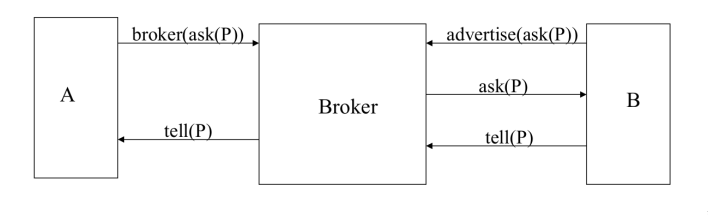
\includegraphics[scale=0.7]{04/cf.png}
  \caption{Communication Facilitators.}
\end{figure}

\cor{Semantica di KQML}{
Precondizioni, postcondizioni e condizioni di completamento descrivono lo stato degli agenti in un linguaggio basato su stati mentali espressi mediante attitudini e descrivono azioni.
}

\nt{Non è fornito un modello semantico per gli stati mentali espressi mediante attituidini.}

\dfn{FIPA ACL}{
  La Foundation for Intelligent Physical Agents (FIPA) è stata fondata con il fine di produrre degli standard per il software per agenti interagenti ed eterogenei e sistemi basati su agenti. FIPA opera attraverso una collaborazione aperta internazionale di organizzazioni associate, aziende, centri di ricerca e università. FIPA ACL è un linguaggio per comunicazione per agenti simile a KQML.
}

\paragraph{KWML vs. FIPA ACL:}

\begin{itemize}
  \item I due linguaggi sono simili alla base. 
  \item Non sono vincolati a un linguaggio per esprimere il contenuto. 
  \item La differenza principale è la semantica. 
  \item Un'altra differenza è la mancanza di primitive di tipo facilitators in FIPA ACL.
\end{itemize}







